\documentclass[border=3pt, tikz]{standalone}
\usepackage{physics}
\usepackage{tikz}
\usepackage[outline]{contour} % glow around text
\usetikzlibrary{calc, arrows.meta}

\tikzset{>=latex} % LaTeX arrow heads
\contourlength{1.35pt}

% Color definitions
\colorlet{xcol}{blue!70!black}
\colorlet{vcol}{green!60!black}
\colorlet{cmcol}{red!70!black}
\colorlet{masscol}{red!50!black}
\colorlet{ellipsecol}{gray!50!black}

% TikZ styles
\tikzstyle{rvec}=[->, xcol, very thick, line cap=round]
\tikzstyle{vvec}=[->, vcol, very thick, line cap=round]
\tikzstyle{CM}=[cmcol, fill=red!80!black!80]
\tikzstyle{mass}=[line width=0.6, draw=masscol, top color=masscol!30, bottom color=masscol!10]
\tikzstyle{ellipse}=[dashed, ellipsecol, thick]
\usetikzlibrary{angles, quotes}

\begin{document}

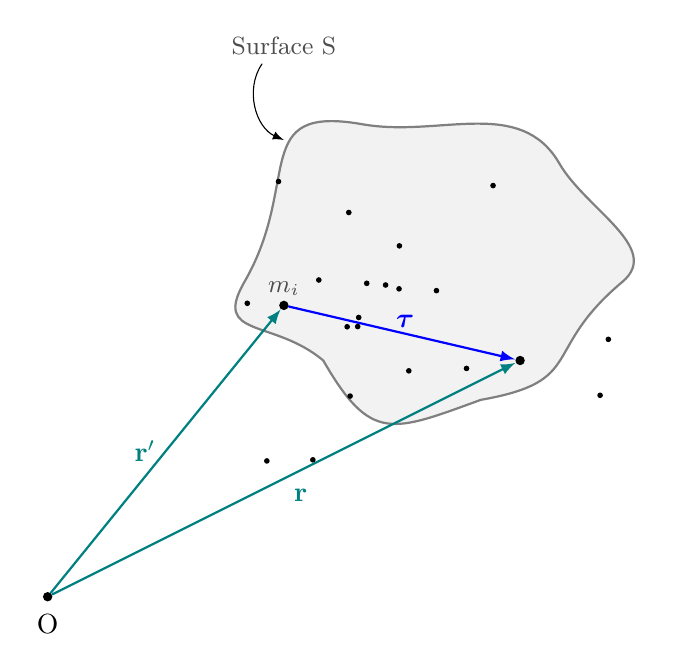
\begin{tikzpicture}[
    line cap=round,
    axis/.style={thick, ->, >=latex, gray},
    mass/.style={circle, fill=black, inner sep=1.2pt},
    vector/.style={thick, ->, teal},
    force/.style={thick, ->, blue},
    annotation/.style={font=\small, black!70},
    surface/.style={thick, gray, fill=gray!10}
    ]

    % Surface Boundary
    \coordinate (A) at (3.5,3);
    \coordinate (B) at (5.5,2.5);
    \coordinate (C) at (7.3,4);
    \coordinate (D) at (6.5,5.5);
    \coordinate (E) at (4,6);
    \coordinate (F) at (2.5,4);

    \draw[surface] (A) to[out=-60, in=200, looseness=1.5] (B)
        to[out=10, in=220, looseness=1.5] (C)
        to[out=40, in=-60, looseness=1] (D)
        to[out=120, in=-10, looseness=1] (E)
        to[out=170, in=60, looseness=1.5] (F)
        to[out=240, in=140, looseness=1.5] cycle;

    % Mass Coordinates
    \node[mass] (O) at (0,0) {};
    \node[mass] (G) at (3,3.7) {};
    \node[mass] (H) at (6,3) {};

    % Randomly Distributed Masses
    % Inside Surface
    \foreach \i in {1,2,...,10}
    {
        \pgfmathsetmacro{\xcoor}{2*rand + 4} % x-coordinate
        \pgfmathsetmacro{\ycoor}{1.5*rand + 4} % y-coordinate
        \draw[fill=black] (\xcoor, \ycoor) circle (0.8pt);
    }

    % Outside Surface
    \foreach \i in {1,2,...,10}
    {
        \pgfmathsetmacro{\xcoor}{2.7*rand + 5} % x-coordinate
        \pgfmathsetmacro{\ycoor}{2.4*rand + 4} % y-coordinate
        \draw[fill=black] (\xcoor, \ycoor) circle (0.8pt);
    }

    % Lines and Vectors
    \draw[vector] (O) -- (G) node[pos=0.5, left] {$\vb{r}'$};
    \draw[force] (G) -- (H) node[pos=0.6, above left] {$\vb*{\tau}$};
    \draw[vector] (O) -- (H) node[pos=0.5, below right] {$\vb{r}$};

    % Surface Label
    \node[annotation] (s) at (3,7) {Surface $\mathrm{S}$};
    \draw[-latex] (s) to[bend right=50] (3,5.8);

    % Labels and Highlights
    \node[above, annotation] at (G) {$m_i$};
    \draw[fill=black] (O) circle (1pt) node[below, shift={(0,-0.1)}] {$\mathrm{O}$};

\end{tikzpicture}

\end{document}